% ============================================================================
\section{Background and Related Work}
\label{sec:background}
% ============================================================================

\paragraph{Why the trigger must filter, and why at a fixed rate.}
The LHC collision rate is \SI{40}{MHz}, far beyond readout capacity. The FPGA-based Level-1 trigger selects about \SI{100}{kHz} within a few microseconds~\cite{atlas_trigger_run3}, using fast detector inputs; eFEX supplies calorimeter trigger objects (TOBs)~\cite{atlas_phase1_tdr}. Our di-tau selection is assigned a $0.5\%$ background-event acceptance budget. The relevant comparison is therefore \emph{signal efficiency at the same background rate}, not threshold-free ROC-AUC (\cref{sec:setting}; trigger context in \cref{app:trigger_context}).

\paragraph{The tau particle and why it is hard to trigger on.}
A tau is a short-lived relative of the electron, produced in processes such as Higgs and $Z$ decays. It decays before reaching the detector. We target its hadronic decays (about $65\%$~\cite{pdg2024}), whose particles leave narrow energy deposits, or \emph{showers}, in the calorimeter. The challenge is that far more common QCD jets can produce similar deposits, especially at low energy. A loose energy cut admits too many jets; a tight cut loses low-energy taus. We therefore use shower shape as well as energy to distinguish them (\cref{app:tau_context}).

\paragraph{Calorimeter inputs.}
Each TOB has a $5\times3\times3$ core tensor spanning four electromagnetic layers (EM0--EM3) and one hadronic layer~\cite{atlas_detector}, plus a finer $12\times12$ EM2 view of the same angular region. For example, the real tau candidate with $\ptTOB=\SI{31.2}{GeV}$ in \cref{fig:calo_input} is represented by five $3\times3$ energy maps (45 values) and 144 EM2-bin energies, not by a photograph. Available scalars are $\ptTOB$, position and an eFEX BDT score. Truth quantities supply labels, loss weights and evaluation variables, never inference inputs; \cref{app:data} specifies their construction.

\begin{figure}[t]
  \centering
  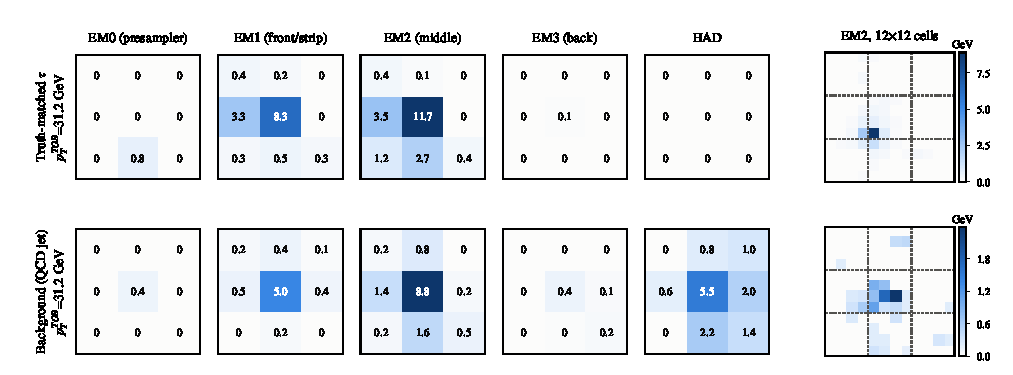
\includegraphics[width=\linewidth]{figures/fig_calo_input.pdf}
  \caption{Calorimeter input of two typical training objects with equal $\ptTOB=\SI{31.2}{GeV}$. Each is chosen at its class median of $\Frac$ (\cref{eq:frac}) and of deposited energy per unit $\ptTOB$. Left: the five $3\times3$ core layers (GeV). Right: EM2 at $12\times12$ granularity; dashed lines mark the towers. The one-prong $\tau$ ($\pttruth=\SI{42.7}{GeV}$) is compact, lies in EM1--EM2 and has no hadronic energy. The jet is wider and deposits much of its energy in HAD.}
  \label{fig:calo_input}
\end{figure}

\paragraph{Prior work.}
This project continues the study of Kernan and Areva Cohen~\cite{kernan2026}, carried out with physicists of the group. They designed physically motivated shower features: per-layer energy sums, core dominance and sparsity (\cref{app:layer_summaries}), and EM2 shape variables such as maxima, peak distances and widths (\cref{app:em2_features}). They then tested how well a $[32,16]$ MLP trained with BCE learns from them. EM1 and EM2 carried most of the separating power, and larger MLPs did not help. Their strongest configuration is shown separately in \cref{fig:results_main}b because its evaluation protocol differs.
On related simulations, \citet{yaari2025trees} compared boosted trees, small MLPs and ResNet-style CNNs for Level-1 $\tau$ selection; the ResNets did not fit the FPGA resources. Tools such as \texttt{hls4ml}~\cite{duarte2018hls4ml} make small fixed-latency networks deployable.

\paragraph{CNNs for detector images.}
Compact convolution--pooling stacks can beat much larger ResNets at low false-positive rates~\cite{ayyar2020cnn}. IceCube uses separate input branches for detector regions of different granularity~\cite{icecube2025cnn}, and strided convolutions can serve as a learned down-sampling front end~\cite{kim2023hotspots}. These ideas shaped our designs in \cref{sec:arch}.

\paragraph{Learning at a fixed operating point.}
Efficiency at a fixed fake rate is a \emph{non-decomposable} objective, because the threshold is itself a quantile of the scores. Such objectives can be optimised with Lagrangian relaxations~\cite{eban2017scalable}. With non-differentiable rate constraints, one can train on smooth surrogates and enforce the constraints from the true rates~\cite{cotter2019proxy}. Our constrained loss (\cref{sec:loss}) follows this separation.
